\section{Plant as sensor}

\subsection{The electronic interface}

The electronic interface is the interface that allows a compute unit to capture and interpret the plant signal and
communication. The interface is a device made by us for this use case. The printed circuit board (PCB)
device is composed of 3 main parts:
\begin{itemize}
    \item The core of the circuit, the microcontroller, an ESP32 Wroom 32
    \item An electronic filter connected using an electrode to the plant
    \item A sound part of the PCB that is including an audio amplifier, a volume knob and a terminal block to connect a speaker
\end{itemize}

The design of the PCB has been done using the open source software Kicad.
As said previously, the circuit contain 3 parts.

The core of the circuit is the computation part, including the microcontroller, an ESP32. All the other
devices of the circuit are connected to the ESP32. The choice to use a devkit has been done 
to ease the electronic conception and to avoid any communication and soldering issue with the MCU\footnote[1]{Microcontroller Unit}.

\begin{figure}[h!]
    \centering
    \includegraphics[width=\textwidth]{images/iop.pdf}
    \caption{The core of the circuit, the microcontroller, an ESP32 Wroom 32. All the other parts of
    circuits are plugged in.} 
    \vspace{0.1cm}
    \label{fig:iop_schematic_main}
\end{figure}

The circuit component that allows us to read data from the plant is the electronic filter.
This filter has been designed by \textit{Jakub Nikonowicz} and \textit{Łukasz Matuszewski} 
from \textit{Politechnika Poznańska}.
Thanks to them, I adapted it for my application on my embedded device. 

\begin{figure}[h!]
    \centering
    \includegraphics[width=\textwidth]{images/iop-plant_filter.pdf}
    \caption{The electronic circuit designed to capture the interaction by analyzing the electronic
    frequency response. The circuit includes 3 resistors, 3 inductors and 3 capacitors as main components} 
    \vspace{0.1cm}
    \label{fig:iop_schematic_filter}
\end{figure}

The last part of the circuit is the sound output/rendering. This circuit includes a small amplifier,
the LM386 from Texas Instruments. The rest of the circuit are components needed in order to 
induce amplification on the signal without creating to many noise and saturation.

\begin{figure}[h!]
    \centering
    \includegraphics[width=\textwidth]{images/iop-audio_circuit.pdf}
    \caption{The sound output part of the circuit that is used to render the sound. 
    This part includes a small amplifier, the LM386. The circuit also includes the components necessary
    to control and handle the amplification (reduce noise and saturation)} 
    \vspace{0.1cm}
    \label{fig:iop_schematic_audio}
\end{figure}


Once the schematic is done, we have to route the tracks. It exists multiple way to route PCB 
(single-sided, double-sided, multiple layers). We choose double sided, 2 layers on each side of the PCB.

\begin{figure}[h!]
    \centering
    \includegraphics[width=\textwidth]{images/iop-routed_pcb.pdf}
    \caption{The routed double sided PCB.} 
    \vspace{0.1cm}
    \label{fig:iop_routed_pcb}
\end{figure}

Kicad also allows us to generated a 3D view of the future PCB. This allows us to imagine what the
PCB will look like when it will be manufactured.
\begin{figure}[h!]
    \centering
    \includegraphics[width=0.8\textwidth]{images/front_iop_3D_view_modified.png}
    \caption{Front 3D rendering of the built PCB. The rendering is done using open source software: Kicad} 
    \vspace{0.1cm}
    \label{fig:front_iop_3D_view_modified}
\end{figure}

\subsection{Human interaction}
\subsubsection{ezaea}
\newpage
\subsubsection{User study}
In the context of the Internet of Things (IoT), this study delves into the nascent field of human-plant interaction, as envisioned by the Internet of Plant project. 
This innovative initiative explores the potential intersections between human actions and botanical entities to create a symbiotic relationship between nature and technology. 
The central inquiry involves imagining a future where plants respond acoustically to physical touch. 
Three distinct plant species—Dypsis lutescens, Pachira glabra, and Dracaena—are employed as subjects to examine user perceptions and interactions within this imagined framework. 
The objective is to contribute to the discourse surrounding the integration of technology and nature by discerning the various ways in which individuals conceptualize and interact with plants as potential musical collaborators.


\subsu{Methodology}

\subsection{Participants}




\subsection{Procedure}

The procedure unfolded in a systematic fashion to facilitate a comprehensive exploration of participants' perceptions and interactions with the envisioned musical plants. Upon welcoming each participant, we presented them with the intriguing premise: "We're in the very near future. You are looking at plants that make music when you physically interact with them (it is not actually the case, but imagine it). Explore their capabilities." This imaginative prompt aimed to elicit uninhibited responses and creative engagement. Subsequently, participants were given the freedom to explore the potential musical capacities of the plants at their own pace. An important aspect of the procedure was our deliberate decision not to provide any guidance or answer questions during the exploration phase, allowing for unfiltered and spontaneous reactions. In instances where participants encountered difficulty initiating exploration, the prompt was reiterated to encourage a more immersive and uninhibited interaction with the conceptualized musical flora. This methodological approach was designed to capture the unmediated and diverse responses of participants as they navigated the uncharted territory of human-plant interaction. Also, we avoided any kind of communication or talking between 2 participants to reduce the potential bias.


\subsection{Materials/Tools}

To proceed and conduct this user study, we choose 3 different plants from 3 different species.

\newpage

\subsubsection{Dracaena}
They project was initially conducted using this specific plant. It has long leaves and fragile perceived trunk but also flexible.

\begin{figure}[h!]
    \centering
    \includegraphics[width=0.42\textwidth, angle=-90]{small_plant.jpg}
    \caption{The N°1 plant is a \textit{Dracaena}.}
    
    \vspace{-0.5cm}
    \label{fig:small_plant}
    \vspace{0.2cm}
\end{figure}




\subsubsection{Pachira glabra}

We chose to use this plant for its large leaves and its wide trunk. This \textit{Pachira} is a bit taller than the \textit{Dracaena} (figure \ref{fig:small_plant}).
\begin{figure}[h!]
    \centering
    \includegraphics[width=0.42\textwidth, angle=-90]{tall_plant_cropped.jpg}
    \caption{The N°2 plant is a \textit{Pachira glabra}.}
    
    \vspace{-0.5cm}
    \label{fig:tall_plant}
    \vspace{0.2cm}
\end{figure}


\newpage

\subsubsection{Dypsis lutescens}

The \textit{Dypsis lutescens} is very different from the two other plants. Indeed, it is composed of many trunks and stems. On top of that, the leaves are numerous and tight.

\begin{figure}[h!]
    \centering
    \includegraphics[width=0.42\textwidth, angle=-90]{fougere_plant.jpg}
    \caption{The N°3 plant is a \textit{Dypsis lutescens}.}
    
    \vspace{-0.5cm}
    \label{fig:fougere_plant}
    \vspace{0.2cm}
\end{figure}



\subsubsection{The experimental space}

The experimental space served as an open canvas for the exploration of human-plant interaction within the Internet of Plant project. While the configuration was not explicitly tailored to the plants, it provided a versatile environment that accommodated the envisioned musical flora. The space featured three distinct levels of height, each corresponding to one of the three plants introduced to participants. 

\begin{figure}[h]
    \centering
    \includegraphics[width=0.42\textwidth]{setup_user_study.jpg}
    \caption{User study space setup. The setup is built from our lab space.}
    
    \vspace{-0.5cm}
    \label{fig:setup_user_study}
    \vspace{0.2cm}
\end{figure}

\section{Data collection}
To capture the nuances of participant interactions with the conceptualized musical plants, a collaborative approach was adopted, involving two researchers to provide dual perspectives. Throughout the exploration phase, both researchers meticulously took notes, documenting the diverse ways in which participants engaged with the three distinct plants. Each note explicitly specified the plant involved in the interaction, ensuring a granular understanding of the responses tied to each botanical entity.

The notes encompassed detailed descriptions of participants' actions, expressions, and verbalizations, aiming to encapsulate the richness of their experiences. The dual-observer strategy facilitated a more comprehensive and triangulated perspective, mitigating potential biases and enhancing the reliability of the recorded data. The collaborative note-taking process served as a valuable means of capturing the multifaceted nature of human-plant interaction within the experimental context, contributing to the depth and richness of the findings in the subsequent analysis.

We defined 5 possible interaction :

\begin{itemize}
    \item Grasp : user uses the whole hand to grab trunk or leaves
    \item Pinch : user uses 2 to 3 digits to grab trunk or leaves
    \item Slide : user uses his/her hand or finger to slide on the plant
    \item Pet : user uses his/her hand to cuddle the plant or to pass through the leaves
    \item Tam Tam : user taps on the plant mainly using the whole hand
\end{itemize}


\section{Results}
Looking at the results, we extracted the table \ref{tab:results}.


\begin{table}[ht]
\begin{tabular}{|l|ll|l|ll|}
\hline
\multirow{2}{*}{Plant/Interaction} & \multicolumn{2}{l|}{Group 1}       & Group 2 & \multicolumn{2}{l|}{Group 3}       \\ \cline{2-6} 
                                   & \multicolumn{1}{l|}{Grasp} & Pinch & Slide   & \multicolumn{1}{l|}{Pet} & Tam Tam \\ \hline
Plant N°1                          & \multicolumn{1}{l|}{4}     & 8     & 4       & \multicolumn{1}{l|}{4}   & 2       \\ \hline
Plant N°2                          & \multicolumn{1}{l|}{9}     & 3     & 3       & \multicolumn{1}{l|}{3}   & 10      \\ \hline
Plant N°3                          & \multicolumn{1}{l|}{10}    & 1     & 5       & \multicolumn{1}{l|}{7}   & 3       \\ \hline
Total                              & \multicolumn{1}{l|}{23}    & 12    & 12      & \multicolumn{1}{l|}{14}  & 15      \\ \hline
\end{tabular}
% \caption*{Plant N°1 : Petite | Plant N°2 : Grande | Plant N°3 : Fougère}
\caption{Raw results extracted from the user study}
\label{tab:results}
\end{table}

\newpage

Regarding the results we drew a graph.


\begin{figure}[ht]
    \centering
    \includegraphics[width=0.42\textwidth]{Images/plant_interaction_chart.png}
    \caption{Bar chart that is extracting the main types of interaction regarding each plants.}
    
    \vspace{-0.5cm}
    \label{fig:setup_user_study}
    \vspace{0.2cm}
\end{figure}

In the end, of the 22 participants, 15 were already familiar with the project and 7 were not.


Looking at the results, the interaction were various depending on the plant. Thus, we can extract main interactions that are linked to the plant type. Looking at tab. \ref{tab:results}, people are more inclined to use their hands as tam tam or grasp the \textit{Pachira glabra}. However, for the \textit{Dracaena} people prefer to pinch the trunk or leave. People decided to grasp whether a pack of trunk or leaves when it came to \textit{Dypsis lutescens}.
This is induced by many factors including the leaves shape, the width of the trunk.


It was observed that when the plants were positioned at higher elevations on the table, individuals tended to engage more with the trunk of the plants. \hl{link to the future graph}

Looking at table \ref{tab:results}, we decided to group interaction. This was done by grouping type of interaction depending on 3 main factors :

\begin{itemize}
    \item The intensity factor : what is the intensity of the interaction (ex : pinch is lighter than grasp)
    \item The spatial factor : what is the interaction displacement.
    \item The duration factor : what is the interaction duration (ex : tam tam is instantaneous).
\end{itemize}

The "Group 1" includes the pinch and grasp interaction. Indeed, looking at the 3 factors we defined, the pinch and grasp are high in intensity and long in duration but people stay still in space.

The "Group 2" includes the slide. The slide interaction is long in time, it moves in space but low in intensity.

Whereas, the "Group 3" includes the pet and Tam Tam. These 2 interactions are really high in intensity, people usually tam tam and pet in different places but those interactions are short in time. 


\begin{figure}[h]
    \centering
    \includegraphics[width=0.42\textwidth]{Images/iop_triangle.png}
    \caption{Graph that is allowing to visualize the possible extracted properties of interactions types. Group 1, 2 and 3 refers to the group in the table \ref{tab:results}.}
    
    \vspace{-0.5cm}
    \label{fig:interaction_type_triangle}
    \vspace{0.2cm}
\end{figure}
\subsection{...}